%!TEX TS-program = pdflatex
% dissertation.tex -- main dissertation file
%
% Wisconsin dissertation template
% Copyright (c) 2008-2009 William C. Benton.  All rights reserved.
%
% This program can redistributed and/or modified under the terms
% of the LaTeX Project Public License Distributed from CTAN
% archives in directory macros/latex/base/lppl.txt; either
% version 1 of the License, or (at your option) any later version.
%
% This program includes other software that is licensed under the
% terms of the LPPL and the Perl Artistic License; see README for details.
%
% You, the user, still hold the copyright to any document you produce
% with this software (like your dissertation).
%

%%% You'll want ``oneside'' for the deposit version, but probably not for any versions that don't need to meet the UW requirements
\documentclass[12pt,oneside,letterpaper]{memoir}

\usepackage{todonotes}
\usepackage{acronym}{glossaries}

% preamble.tex -- packages to include
%
% Wisconsin dissertation template
% Copyright (c) 2008 William C. Benton.  All rights reserved.
%
% This program can redistributed and/or modified under the terms
% of the LaTeX Project Public License Distributed from CTAN
% archives in directory macros/latex/base/lppl.txt; either
% version 1 of the License, or (at your option) any later version.
%
% This program includes other software that is licensed under the
% terms of the LPPL and the Perl Artistic License; see README for details.
%
% You, the user, still hold the copyright to any document you produce
% with this software (like your dissertation).

%% You should use natbib
\IfFileExists{natbib.sty}{%
\usepackage{natbib}%
}{}

%% You probably need appendix, if you want appendices
\IfFileExists{appendix.sty}{%
\usepackage{appendix}%
}{}

%% the spacing in memoir is weird, you'll need to use this
\DisemulatePackage{setspace}
\usepackage[onehalfspacing]{setspace}

%% List setup; the ``hanglist`` environment will allow you to have
%% nicely-typeset enumerated lists (i.e. with the numbers hanging in
%% the margins).  You need at least version 2.1 of enumitem.sty.  If
%% you don't have enumitem installed at all, hanglist will just be an
%% alias for enumerate.
\IfFileExists{enumitem.sty}{%
\usepackage[loadonly]{enumitem}[2007/06/30]%
\newlist{hanglist}{enumerate}{1}% 
\setlist[hanglist]{label=\arabic*.}%
\setlist[hanglist,1]{leftmargin=0pt}%
}{%
\newenvironment{hanglist}{\begin{enumerate}}{\end{enumerate}}%
}

%% Comment out any of these that you don't want
\usepackage{amssymb}
\usepackage{amsmath}
\usepackage{amsthm}
%\usepackage{theorem}
\usepackage{hyperref}

\IfFileExists{mathpartir.sty}{%
\usepackage{mathpartir}%
}{}

%%%%% LISTINGS package and setup
\IfFileExists{listings.sty}{%
\usepackage{listings}%
}{}



%% Get rid of ugly borders around PDF hyperlinks (e.g. for cross-references, bib entries, or URLs)
\hypersetup{pdfborder = 0 0 0}

%% You want microtype.
\IfFileExists{microtype.sty}{%
\usepackage[protrusion=true,expansion=true]{microtype}%
}{}

%\pagestyle{thesisdraft}

% Surround parts of graphics with box
\usepackage{boxedminipage}

%% booktabs (thx to Nate Rosenblum for bringing this beautiful package
%% to my attention)
\IfFileExists{booktabs.sty}{%
\usepackage{booktabs}%
}{}

% This is now the recommended way for checking for PDFLaTeX:
\usepackage{ifpdf}

%% Avoid ugly "Type 3" fonts
\usepackage{lmodern}
\usepackage[LY1]{fontenc}

%% Substitute your favorite serif and sans fonts here....
\IfFileExists{tgpagella.sty}{%
% TeX Gyre pagella, like Palatino
\usepackage{tgpagella}%
}{}

\usepackage[LY1]{eulervm}

\ifpdf
\usepackage[pdftex]{graphicx}
\else
\usepackage{graphicx}
\fi

\usepackage{makeidx}
\makeindex

{\theoremstyle{plain}
\newtheorem{thm}{Theorem}[chapter]
\newtheorem{cor}[thm]{Corollary}
\newtheorem{define}[thm]{Definition}
\newtheorem{exmpl}[thm]{Example}
}
{\theoremstyle{remark}
\newtheorem{rmk}[thm]{Remark}
}

\newtheoremstyle{customsty1}
{3pt}%
{3pt}%
{}% --- body font
{}% --- indent amount
{\bfseries}% --- Theorem head font
{:}% --- Punctuation after head
{.5em}% --- space after head
{}% --- theorem head spec (can be left empty, meaning 'normal')

% Define 'newtheorems' that use ``customsty1''
{\theoremstyle{customsty1} 
}


%%% NB: the ``deposit'' chapter- and page- styles should conform to UW
%%% requirements.  If you are producing a pretty version of your
%%% dissertation for web use later, you will certainly want to make
%%% your own chapter and page styles.

\makechapterstyle{deposit}{%
  \renewcommand{\chapterheadstart}{}
  \renewcommand{\printchaptername}{}
  \renewcommand{\chapternamenum}{}
  \renewcommand{\printchapternum}{\parbox{2em}{\MakeLowercase{\Large\scshape\thechapter{}}} }
  \renewcommand{\afterchapternum}{}
  \renewcommand{\printchaptertitle}[1]{%
  \raggedright\Large\scshape\MakeLowercase{##1}}
  \renewcommand{\afterchaptertitle}{%
  \vskip\onelineskip \hrule\vskip\onelineskip}
}

\makepagestyle{deposit}
 
\makeatletter
 
\renewcommand{\chaptermark}[1]{\markboth{#1}{}}
\renewcommand{\sectionmark}[1]{\markboth{#1}{}}
 
\makeevenfoot{deposit}{}{}{}
\makeoddfoot{deposit}{}{}{}
\makeevenhead{deposit}{\thepage}{}{}
\makeoddhead{deposit}{}{}{\thepage}
\makeatother

%%% set up page numbering for chapter pages to satisfy UW requirements
%%% NB: You will want to delete until the ``SNIP'' mark if you are
%%% making a ``nice'' copy
\copypagestyle{chapter}{plain}
\makeoddfoot{chapter}{}{}{}
\makeevenhead{chapter}{\thepage}{}{}
\makeoddhead{chapter}{}{}{\thepage}
%%% SNIP

%%% bib nonsense
\makeatletter
\newenvironment{wb-bib}[1]{%
  \chapter*{references}
\ifnobibintoc\else 
\phantomsection 
\addcontentsline{toc}{chapter}{References} 
\fi 
\prebibhook
  \begin{bibitemlist}{#1}}{\end{bibitemlist}\postbibhook}

\AtBeginDocument{%
  \@ifpackageloaded{natbib}{% natbib is loaded
    \addtodef{\endthebibliography}{}{\vskip-\lastskip\postbibhook}
    \@ifpackagewith{natbib}{sectionbib}{% with sectionbib option
      \renewcommand{\bibsection}{\@memb@bsec}}%
      {\renewcommand{\bibsection}{\@memb@bchap}}}%
  {}
  \@ifpackagewith{chapterbib}{sectionbib}{%
    \renewcommand{\sectionbib}[2]{}
    \renewcommand{\bibsection}{\@memb@bsec}}{}
}
\makeatother

% defs.tex -- wbepi environment for chapter epigraphs and other useful defs.
%
% Wisconsin dissertation template
% Copyright (c) 2008 William C. Benton.  All rights reserved.
%
% This program can redistributed and/or modified under the terms
% of the LaTeX Project Public License Distributed from CTAN
% archives in directory macros/latex/base/lppl.txt; either
% version 1 of the License, or (at your option) any later version.
%
% This program includes other software that is licensed under the
% terms of the LPPL and the Perl Artistic License; see README for details.
%
% You, the user, still hold the copyright to any document you produce
% with this software (like your dissertation).


%% put lstnewenvironment declarations here, if you're using listings

%% end lstnewenvironment declarations

%% I put convenience definitions that will go in several chapters here

%%%%% begin convenience definitions

\makeatletter
\newcommand{\wb@episource}{}
\newenvironment{wbepi}[1]{\begin{quote}\renewcommand{\wb@episource}{#1}\itshape}{\par\upshape \raggedleft --- \textsc{\wb@episource}\\ \end{quote}}
\makeatother

%%%%% SVN
\IfFileExists{svn-multi.sty}{%
\usepackage{svn-multi}%
%%% Uncomment the second one and comment out the first one if you want
%%% to include subversion revision information in each file.
\newcommand{\vcinfo}{}%
%\newcommand{\vcinfo}{\begin{centering}\fbox{\fbox{\parbox{5in}{Author: \svnauthor\\Revision: \svnfilerev\\Last changed on: \svnfiledate\\URL: \svnkw{HeadURL}}}}\\[1em]\end{centering}}%
}{%
\newcommand{\svnidlong}[4]{}%
\newcommand{\svnfilerev}{}%
\newcommand{\svnauthor}{}%
\newcommand{\svnfiledate}{}%
\newcommand{\svnkw}{}%
\newcommand{\vcinfo}{}%
}

%%%%% end convenience definitions

% thesisdefs.tex

% This is mostly adapted from withesis.cls.  The original copyright
% notice for withesis.cls follows, preceded by two percent signs (%%):

%% withesis.cls
%% LaTeX Style file for the University of Wisconsin-Madison Thesis Format
%% Adapted from the Purdue University Thesis Format
%% Originally by Dave Kraynie
%% Edits by Darrell McCauley
%% Adapted to UW-Madison format by Eric Benedict  (Noted with <EB>)
%% Updated to LaTeX2e by Eric Benedict 24 July 00
%% 
%%=============================================================================
%% Licensed under the Perl Artistic License.
%% see: http://www.ctan.org/tex-archive/help/Catalogue/licenses.artistic.html
%% for more info...
%%=============================================================================

% withesis.cls is available from CTAN.  The modifications to this file
% are also licensed under the Perl Artistic License.

% --wb, 2008

\makeatletter

\newcounter {tocpage}
\newcounter {lofpage}
\newcounter {lotpage}
\newcounter {listofheading}

\newcommand\@thesistitlesmallskip{0.2in}
\newcommand\@thesistitlemedskip{0.4in} 
\newcommand\@thesistitlebigskip{0.8in} 
\newcommand{\degree}[1]{\gdef\@degree{#1}}
\newcommand{\project}{\gdef\@doctype{A masters project report}}
\newcommand{\prelim}{\gdef\@doctype{A preliminary report}}
\newcommand{\thesis}{\gdef\@doctype{A thesis}}
\newcommand{\dissertation}{\gdef\@doctype{A dissertation}}
\newcommand{\department}[1]{\gdef\@department{(#1)}}

\newenvironment{titlepage}
 {\@restonecolfalse\if@twocolumn\@restonecoltrue\onecolumn
  \else \newpage \fi \thispagestyle{empty}
% \c@page\z@ -- deleted: count title page in thesis
}{\if@restonecol\twocolumn \else \newpage \fi}

\gdef\@degree{Doctor of Philosophy}    %Default is PhD
\gdef\@doctype{A dissertation }        %Default is dissertation

\gdef\@department{Nuclear Engineering \& Engineering Physics} 
\gdef\@defensedate{16 August 2021}
\gdef\@committee{
  \setstretch{1.0}
  \footnotesize
  Sunil S. Chirayath, Associate Professor, Nuclear Engineering, Texas A\&M University\\
  Douglass L. Henderson, Spangler Professor, Nuclear Engineering \& Engineering Physics\\
  Benjamin A. Lindley, Assistant Professor, Nuclear Engineering \& Engineering Physics\\
  Robert D. Nowak, Nosbusch Professor, Electrical \& Computer Engineering\\
  Paul P.H. Wilson, Grainger Professor, Nuclear Engineering \& Engineering Physics
  }

\renewcommand{\maketitle}{%
  \begin{titlepage}
%-----------------------------------------------------------------------------
% -- The thesis office doesn't like thanks on title page.  Put it in
% -- the acknowledgments.  This is here so you don't have to change
% -- your titlepage when converting from report style. -> from Purdue, but I
%        left it here since it seems compatible with UW-Madison, Eric
%-----------------------------------------------------------------------------
    \def\thanks##1{\typeout{Warning: `thanks' deleted from thesis titlepage.}}
    \let\footnotesize\small \let\footnoterule\relax \setcounter{page}{1}
    \begin{center}
      {\textbf{\expandafter\expandafter{\Large \@title}}} \\[\@thesistitlesmallskip]
       by \\[\@thesistitlesmallskip]
      {\Large \@author} \\[\@thesistitlemedskip]
      \@doctype submitted in partial fulfillment of \\ the requirements for the degree of \\[\@thesistitlemedskip]
      {\Large \@degree} \\[\@thesistitlesmallskip]
      {\large \@department} \\[\@thesistitlesmallskip]
      at the \\[\@thesistitlesmallskip]
      {\large UNIVERSITY OF WISCONSIN--MADISON} \\[\@thesistitlesmallskip]
      {\large \@date}
      \\[\@thesistitlebigskip]
    \end{center}
    \hspace*{-0.5cm}Date of final oral examination: \@defensedate \\[\@thesistitlesmallskip]
    \hspace*{-0.5cm}{\small The dissertation is approved by the following members of the Final Oral Committee:}\\
    \@committee
  \end{titlepage}
  \setcounter{footnote}{0}
  \setcounter{page}{1} %title page is NOT counted
  \let\thanks\relax
  \let\maketitle\relax \let\degree\relax \let\project\relax \let\prelim\relax
  \let\department\relax
  \gdef\@thanks{}\gdef\@degree{}\gdef\@doctype{}
  \gdef\@department{}
  %\gdef\@author{}\gdef\@title{}
}


%=============================================================================
% ABSTRACT
%=============================================================================
% The abstract should begin with two single-spaced lines describing
% the author and title in a standard format.  After these lines comes
% the standard abstract.
%=============================================================================
\def\abstract{
  \chapter*{Abstract}
  \addcontentsline{toc}{chapter}{Abstract}
  \relax\markboth{Abstract}{Abstract}}
\def\endabstract{\par\newpage}


%=============================================================================
% UMI ABSTRACT
%=============================================================================
% The UMI abstract should begin with the author and title in a standard format.
% After the author comes the advisor and university. After these lines comes
% a bunch of double spaced text to make up the standard abstract.
% After the abstract, the advisor's approval signature follows.
% This page is not numbered and is delivered seperately to the thesis office.
%=============================================================================

\def\advisortitle#1{\gdef\@advisortitle{#1}}
\def\advisorname#1{\gdef\@advisorname{#1}}
\gdef\@advisortitle{Professor}
\gdef\@advisorname{Cheer E.\ Place}

\def\umiabstract{
             \thispagestyle{empty}
                  \addtocounter{page}{-1}
                \begin{center}
                  {\textbf{\expandafter\uppercase\expandafter{\@title}}}\\
                  \vspace{12pt}
                  \@author \\
                  \vspace{12pt}
                  Under the supervision of \@advisortitle\ \@advisorname\\
                  At the University of Wisconsin-Madison
                \end{center}
}

\def\endumiabstract{\vfill \hfill\@advisorname\par\newpage}


%============================================================================
% VERBATIMFILE
%============================================================================
% \verbatimfile{<filename>}    for verbatim inclusion of a file
% - Note that the precise layout of line breaks in this file is important!
% - added the \singlespace - EB
%============================================================================
\def\verbatimfile#1{\begingroup \singlespace
                    \@verbatim \frenchspacing \@vobeyspaces
                    \input#1 \endgroup
}


%=============================================================================
% SEPARATOR Pages
%   Creates a blank page with a text centered horizontally and vertically.
%   The page is neither counted nor numbered.
%   These pages are required in the thesis format before sections such
%   as appendices, vita, bibliography, etc.
%=============================================================================
\def\separatorpage#1{
  \newpage
  \thispagestyle{empty}
  \addtocounter{page}{-1}
  \null
  \vfil\vfil
  \begin{center}
    {\textbf{#1}}
  \end{center}
  \vfil\vfil
  \newpage}


%=============================================================================
% COPYRIGHTPAGE
%=============================================================================
% The copyright must do the following:
% - start a new page with no number
% - place the copyright text centered at the bottom.
%=============================================================================
\def\copyrightpage{
  \newpage
  \thispagestyle{empty}    % No page number
  \addtocounter{page}{-1}
  \chapter*{}            % Required for \vfill to work
  \begin{center}
   \vfill
   \copyright\ Copyright by \@author\ \@date\\
   All Rights Reserved
  \end{center}}


%=============================================================================
% GLOSSARY
%=============================================================================
% The glossary environment must do the following:
% - produce the table of contents entry for the glossary
% - start a new page with GLOSSARY centered two inches from the top
%=============================================================================
%\def\glossary{
%  \chapter*{GLOSSARY}
%  \addcontentsline{toc}{chapter}{Glossary}}
%\def\endglossary{\par\newpage}

%=============================================================================
% NOMENCLATURE
%=============================================================================
% The nomenclature environment must do the following:
% - produce the table of contents entry for the nomenclature section
% - start a new page with NOMENCLATURE centered two inches from the top
%=============================================================================
\def\nomenclature{\separatorpage{DISCARD THIS PAGE}
  \chapter*{Nomenclature}
  \addcontentsline{toc}{chapter}{NOMENCLATURE}}
\def\endnomenclature{\par\newpage}

%=============================================================================
% CONVENTIONS
%=============================================================================
% The conventions environment must do the following:
% - produce the table of contents entry for the nomenclature section
% - start a new page with CONVENTIONS centered two inches from the top
%=============================================================================
\def\conventions{\separatorpage{DISCARD THIS PAGE}
  \chapter*{Conventions}
  \addcontentsline{toc}{chapter}{CONVENTIONS}}
\def\endconventions{\par\newpage}


%=============================================================================
% COLOPHON
%=============================================================================
% The colophon environment must do the following:
% - produce the table of contents entry for the nomenclature section
% - start a new page with COLOPHON centered two inches from the top
%=============================================================================
\def\colophon{\separatorpage{DISCARD THIS PAGE}
  \chapter*{Colophon}
  \addcontentsline{toc}{chapter}{Colophon}}
\def\endcolophon{\par\newpage}

%=============================================================================
% LIST OF SYMBOLS
%=============================================================================
% The list of symbols environment must do the following:
% - produce the table of contents entry for the list of symbols section
% - start a new page with LIST OF SYMBOLS centered two inches from the top
%=============================================================================
\def\listofsymbols{\separatorpage{DISCARD THIS PAGE}
  \eject
  \chapter*{LIST OF SYMBOLS}
  \addcontentsline{toc}{chapter}{LIST OF SYMBOLS}}
\def\endlistofsymbols{\par\newpage}

%=============================================================================
% VITA
%=============================================================================
% The vita environment must do the following:
% - produce a separator page with the word vita centered
% - produce the table of contents entry for the vita
% - start a new page with VITA centered two inches from the top
%=============================================================================
\def\vita{
%  \separatorpage{VITA}         % UW doesn't require this EB
  \chapter*{VITA}
  \addcontentsline{toc}{chapter}{VITA}}
\def\endvita{\par\newpage}

%=============================================================================
% ACKNOWLEDGMENTS
%=============================================================================
% The acknowledgments environment must do the following:
% - start a new page with ACKNOWLEDGMENTS centered two inches from the top
%=============================================================================
\def\acks{
  \chapter*{Acknowledgments}
}
\def\endacks{\par\newpage}

%=============================================================================
% DEDICATION
%=============================================================================
% The dedication environment must do the following:
% - start a new page
% - center the text vertically
% - include the text in a center environment
%=============================================================================
%\def\dedication{
%  \newpage
%  \null\vfil
%  \begin{center}}
%\def\enddedication{\end{center}\par\vfil\newpage}

\def\dedication{
  \newpage
  \null\vfil
  }
\def\enddedication{\par\vfil\newpage}
%=============================================================================
% DATE
%=============================================================================
%\def\today{\ifcase\month\or
  %January\or February\or March\or April\or May\or June\or
  %July\or August\or September\or October\or November\or December\fi
  %\space\number\day, \number\year}
\newcount\@testday
\def\today{\@testday=\day
  \ifnum\@testday>30 \advance\@testday by -30
  \else\ifnum\@testday>20 \advance\@testday by -20
  \fi\fi
  \number\day\ \
  \ifcase\month\or
    January \or February \or March \or April \or May \or June \or
    July \or August \or September \or October \or November \or December
    \fi\ \number\year
}


%  Single counter for theorems and theorem-like environments:
\newtheorem{theorem}{Theorem}[chapter]
\newtheorem{assertion}[theorem]{Assertion}
\newtheorem{claim}[theorem]{Claim}
\newtheorem{conjecture}[theorem]{Conjecture}
\newtheorem{corollary}[theorem]{Corollary}
\newtheorem{definition}[theorem]{Definition}
\newtheorem{example}[theorem]{Example}
\newtheorem{figger}[theorem]{Figure}
\newtheorem{lemma}[theorem]{Lemma}
\newtheorem{prop}[theorem]{Proposition}
\newtheorem{remark}[theorem]{Remark}

%=============================================================================
% TABLE OF CONTENTS; LIST OF FIGURES; LIST OF TABLES
%=============================================================================
% In report style, \tableofcontents, \listoffigures, etc. are always
% set in single-column style.  @restonecol is used to keep track of
% whether we need to switch back to double column style after the toc.
%
% The only known problem now is that the first page with the new
% layout is too long.  The problem seems to be that the change to
% textheight doesn't take place on the first page.  Even if it's the
% first line in the table of contents macro.  Presumably the same
% problem also occurs in the lof and lot.
%
% I'm taking a shot at fixing the problem by dropping in a throw-away
% page between the change to the height parameters and the start of
% the chapter.  Isn't elegance wonderful?
%
%=============================================================================

% \def\@tableof#1#2#3#4#5{
% { % limit scope of following declarations!!
%   \@restonecolfalse\if@twocolumn\@restonecoltrue\onecolumn\fi
%   \addtolength{\textheight}{-40pt}       % -24-16
%   \addtolength{\majorheadskip}{-40pt}    % -24-16
%   \addtolength{\headheight}{52pt}        %  36+16
%   \addtolength{\headsep}{-12pt}          % -12
%   \separatorpage{DISCARD THIS PAGE}
%   \chapter*{#1}
%   #5
%   \relax\markboth{#1}{#1}
%   \hbox to \hsize{#2 \hfil Page}
%   \singlespace
%   \setcounter{#3}{0}
%   \setcounter{listofheading}{1}  % change from 0 to 1 by mccauley, 14may93
%   \def\@oddhead{\vbox to \headheight{\vspace{4pt}
%     \hbox to \hsize{\hfil\textrm{\thepage}} \vfil
%     \ifnum\value{#3}=1
%       \ifnum\value{listofheading}=2
%         \hbox to \hsize{Appendix\hfil} \vspace{4pt} \fi
%       \ifnum\value{listofheading}=1
%         \stepcounter{listofheading} \fi
%       \hbox to \hsize{#2 \hfil Page}
%     \else
%       \setcounter{#3}{1}
%     \fi}}
%   \def\@evenhead{\vbox to \headheight{\vspace{4pt}
%     \hbox to \hsize{\textrm{\thepage}\hfil} \vfil
%     \ifnum\value{#3}=1
%       \ifnum\value{listofheading}=2
%         \hbox to \hsize{Appendix\hfil} \vspace{4pt} \fi
%       \ifnum\value{listofheading}=1
%         \stepcounter{listofheading} \fi
%       \hbox to \hsize{#2 \hfil Page}
%     \else
%       \setcounter{#3}{1}
%     \fi}}
%   \@starttoc{#4}  \if@restonecol\twocolumn\fi
%   \newpage
% }}
% 
% \def\tableofcontents{\@tableof{TABLE OF CONTENTS}{}{tocpage}{toc}{}}
% 
% \def\listoffigures{
%   \@tableof{LIST OF FIGURES}{Figure}{lofpage}{lof}
%   {\protect\addcontentsline{toc}{chapter}{LIST OF FIGURES}}}
% 
% \def\listoftables{
%   \@tableof{LIST OF TABLES}{Table}{lotpage}{lot}
%   {\protect\addcontentsline{toc}{chapter}{LIST OF TABLES}}}

%=============================================================================
% BIBLIOGRAPHY
%=============================================================================
% The thebibliography environment executes the following commands:
%
%  o start a new 'chapter' with BIBLIOGRAPHY as the heading
%  o produce a separator page for the bibliography
%
%  \def\newblock{\hskip .11em plus .33em minus -.07em} --
%      Defines the `closed' format, where the blocks (major units of
%      information) of an entry run together.
%
%  \sloppy  -- Used because it's rather hard to do line breaks in
%      bibliographies,
%
%  \sfcode`\.=1000\relax --
%      Causes a `.' (period) not to produce an end-of-sentence space.
%=============================================================================
% \altbibtitle
%   The default title for the References chapter is ``LIST OF REFERENCES''
%   Since some people prefer ``BIBLIOGRAPHY'', the command
%   \altbibtitle has been added to change the chapter title.
%   This command does nothing more than change REFERENCES to BIBLIOGRAPHY
%============================================================================
\def\@bibchaptitle{Bibliography}
\def\altbibtitle{\def\@bibchaptitle{Bibliography}}
\def\thebibliography#1{
  %\separatorpage{\@bibchaptitle}
  \global\@bibpresenttrue
  \chapter*{\@bibchaptitle\markboth{\@bibchaptitle}{\@bibchaptitle}}
  \addcontentsline{toc}{chapter}{\@bibchaptitle}
  \vspace{0.375in}    % added to match 4 line requirement
  \interlinepenalty=10000 % added to prevent breaking of bib entries
  \singlespace\list
  {[\arabic{enumi}]}{\settowidth\labelwidth{[#1]}\leftmargin\labelwidth
    \advance\leftmargin\labelsep \usecounter{enumi}}
  \def\newblock{\hskip .11em plus .33em minus -.07em}
  \sloppy
  \sfcode`\.=1000\relax}
\let\endthebibliography=\endlist



\makeatother

\newacronym{UW}{UW}{University of Wisconsin}
\newacronym{US}{US}{United States}
\newacronym{DHS}{DHS}{Department of Homeland Security}
\newacronym{DNDO}{DNDO}{Domestic Nuclear Detection Office}
\newacronym{NTNFC}{NTNFC}{National Technical Nuclear Forensics Center}
\newacronym{UOC}{UOC}{uranium ore concentrate}
\newacronym{SNM}{SNM}{special nuclear material}
\newacronym{SNF}{SNF}{spent nuclear fuel}
\newacronym{AI}{AI}{artificial intelligence}
\newacronym{ROC}{ROC}{receiver operating characteristics}
\newacronym{SVR}{SVR}{support vector regression}
\newacronym{SVM}{SVM}{support vector machine}
\newacronym{ORIGEN}{ORIGEN}{Oak Ridge Isotope GENeration}
\newacronym{ORIGEN-ARP}{ORIGEN-ARP}{ORIGEN-Automatic Rapid Processing}
\newacronym{INDEPTH}{INDEPTH}{INverse DEPletion THeory}
\newacronym{GADRAS}{GADRAS}{GAmma Detector Response and Analysis Software}
\newacronym{i.i.d.}{i.i.d.}{independent and identically distributed}
\newacronym{DRF}{DRF}{detector response function}
\newacronym{MAPE}{MAPE}{mean absolute percentage error}
\newacronym{RMSE}{RMSE}{root-mean-squared error}
\newacronym{AGR}{AGR}{advanced gas reactor}
\newacronym{BWR}{BWR}{boiling water reactor}
\newacronym{PWR}{PWR}{pressurized water reactor}
\newacronym{CANDU}{CANDU}{Canada deuterium uranium}
\newacronym{VVER}{VVER}{water-water energetic reactor}
\newacronym{SFCOMPO}{SFCOMPO}{spent fuel isotopic composition}
\newacronym{CHTC}{CHTC}{Center for High Throughput Computing}
\newacronym{PCA}{PCA}{principal components analysis}
\newacronym{ICA}{ICA}{independent components analysis}
\newacronym{PLS}{PLS}{partial least squares}
%\newacronym{}{}{}


\clearpage\pagenumbering{roman}  % This makes the page numbers Roman (i, ii, etc)

\title{My Awesome Title}
\author{Arrielle C.~Opotowsky}
\department{Engineering Physics}

\date{2017}

\begin{document}

\listoftodos

%%% Uncomment the following if your .bib contains references that you will not 
%%% explicitly cite, but that should be in the final bibliography:
\nocite{*}

\ifpdf
\DeclareGraphicsExtensions{.pdf, .jpg, .tif}
\else
\DeclareGraphicsExtensions{.eps, .jpg}
\fi

\maketitle

\svnidlong{$LastChangedBy$}{$LastChangedRevision$}{$LastChangedDate$}{$HeadURL: http://freevariable.com/dissertation/branches/diss-template/frontmatter/frontmatter.tex $}
\vcinfo{}

%%% SOME OF THIS CODE IS ADAPTED FROM THE VENERABLE withesis.cls

% COPYRIGHT PAGE
%  - To include a copyright page use \copyrightpage
\copyrightpage

% DEDICATION
\begin{dedication}
	\emph{Please insert your dedication here.}
\end{dedication}

%% BEGIN PAGESTYLE

%%% You can pick a pagestyle if you want; see the memoir class
%%% documentation for more info.  The default ``deposit'' option meets
%%% the UW thesis typesetting requirements but is probably
%%% unsatisfactory for making a version of your dissertation that
%%% won't be deposited to the graduate school (e.g. for web or a nice
%%% printed copy)

\chapterstyle{deposit}
\pagestyle{deposit}


% ACKNOWLEDGMENTS
\begin{acks}
This proposal would not be possible with the wisdom and patience of my advisor,
Paul Wilson. I honestly don't have words for how grateful I am to you.  I'm
also appreciative of the CNERG community for technical and non-technical
assistance; may quiche recipes be forever shared during important phone calls.
Kelly Burton and Max Lagally have invested much effort into my success and
convinced me that graduate school was the right path for me---more than once.
My GERS friends have given me so much in and out of school, especially Jos\'e
Roberto, Richard, and Chandler.  I have also received generous funding from the
National Science Foundation and the Department of Homeland Security.

Mountains of personal support motivated me here and kept me here, which I do
not take for granted. Steven W. Harrell, my chosen family, inspired me to get
all my KSAs, no matter where I wanted to find them. The "If you're gonna be
dumb, you gotta be tough" mentality hilariously applies to a PhD program.
Robin, you have been such a light in my life for over a decade and always
remind me why I came back to grad school.  And to my friends for 15 years,
thanks for keeping in touch despite the gaps.  Denise and April, it's been
amazing to watch your wonderful transformations. Ruthie, you push me to be
fierce, spittin' truths and slaying your way through life.  Maurice, thanks for
the help when I was struggling. Lou, thanks for being one of my best friends
and sources of laugh lines. Liz, I love finding your inspirational notes around
my home and thanks for all the meals. For endlessly encouraging my academic
pursuits, I'm appreciative of my California family, Mel, Bonnie, Joelle, and
Jamie. Finally, my Madison family has blessed me in countless ways: Shan,
Ninja, Peter, Drax, Heather, Burnie, Marit, Sarah, James, BLou, Fetal, Matt, 


\end{acks}

% CONTENTS, TABLES, FIGURES
\renewcommand{\printtoctitle}[1]{\chapter*{#1}}
\renewcommand{\printloftitle}[1]{\chapter*{#1}}
\renewcommand{\printlottitle}[1]{\chapter*{#1}}

\renewcommand{\tocmark}{}
\renewcommand{\lofmark}{}
\renewcommand{\lotmark}{}

\renewcommand{\tocheadstart}{}
\renewcommand{\lofheadstart}{}
\renewcommand{\lotheadstart}{}

\renewcommand{\aftertoctitle}{}
\renewcommand{\afterloftitle}{}
\renewcommand{\afterlottitle}{}

\renewcommand{\cftchapterfont}{\normalfont} 
\renewcommand{\cftsectionfont}{\itshape} 
\renewcommand{\cftchapterpagefont}{\normalfont} 
\renewcommand{\cftchapterpresnum}{\bfseries} 
\renewcommand{\cftchapterleader}{} 
\renewcommand{\cftsectionleader}{} 
\renewcommand{\cftchapterafterpnum}{\cftparfillskip} 
\renewcommand{\cftsectionafterpnum}{\cftparfillskip} 

% \captionnamefont{\small\sffamily} 
% \captiontitlefont{\small\sffamily} 

% \renewcommand{\contentsname}{contents}
% \renewcommand{\listfigurename}{list of figures}
% \renewcommand{\listtablename}{list of tables}

\tableofcontents

\clearpage
\listoftables

\clearpage
\listoffigures

\clearpage
% NOMENCLATURE
% \begin{conventions}
% % \begin{description}
% % \item{\makebox[0.75in][l]{term}
% %        \parbox[t]{5in}{definition\\}}
% % \end{description}
% \input{conventions}
% \end{conventions}

%% The UW graduate school no longer wants a UMI abstract page
%% Should you need one for some reason, uncomment the following
%% lines.  Thanks to Matt Fredrikson for reporting this!

% \advisorname{Gottlob Frege}
% \advisortitle{Professor}
% \begin{umiabstract}
%  Nuclear forensics is a nuclear security capability that is broadly defined as
material attribution in the event of a nuclear incident.  Improvement and
research is needed for both technical and non-technical components of this
process.  One such technical area is the provenance of non-detonated \gls{SNM};
studied here is \gls{SNF}, which is applicable in a scenario involving the
unlawful use of commercial byproducts from nuclear power reactors.  The
experimental process involves measuring known forensics signatures to ascertain
the reactor parameters that produced the material. Knowing these assists in
locating the source of the material. This work is proposing the use of
statistical methods to determine these quantities instead of empirical
relationships. 

The purpose of this work is to probe to what extent this method is feasible.
Thus, two experiments have been designed, using simulated nuclide measurements
as observations and reactor operation parameters as the prediction goals.
First, machine learning algorithms are employed with full-knowledge training
data, i.e., nuclide vectors directly from simulations.  Second, this workflow
is performed on reduced-knowledge training data, analgous to a detector that
can only measure certain radionuclides. The results are evaluated using the
performance of the reactor parameter predictions.

The reactor parameters of interest are the reactor type and three quantities of
interest describing the \gls{SNF}: burnup, initial U235 enrichment, and time
since irradiation. The algorithms used to predict these quantities are
\textit{k}-nearest neighbors, decision trees, and \gls{MLL} calculations. The
first experiment predicts all of these quantities well using the three
algorithms, except for the case where \textit{k}-nearest neighbors is
predicting time since irradiation. The second experiment has widely varying
results, but two consistent themes: the methods predict burnup very well and
enrichment poorly.

This approach is an exploratory study using simple algorithms. Even so, the
results are overall promising and warrant further study.


% \end{umiabstract}

\begin{abstract}
  Nuclear forensics is a nuclear security capability that is broadly defined as
material attribution in the event of a nuclear incident.  Improvement and
research is needed for both technical and non-technical components of this
process.  One such technical area is the provenance of non-detonated \gls{SNM};
studied here is \gls{SNF}, which is applicable in a scenario involving the
unlawful use of commercial byproducts from nuclear power reactors.  The
experimental process involves measuring known forensics signatures to ascertain
the reactor parameters that produced the material. Knowing these assists in
locating the source of the material. This work is proposing the use of
statistical methods to determine these quantities instead of empirical
relationships. 

The purpose of this work is to probe to what extent this method is feasible.
Thus, two experiments have been designed, using simulated nuclide measurements
as observations and reactor operation parameters as the prediction goals.
First, machine learning algorithms are employed with full-knowledge training
data, i.e., nuclide vectors directly from simulations.  Second, this workflow
is performed on reduced-knowledge training data, analgous to a detector that
can only measure certain radionuclides. The results are evaluated using the
performance of the reactor parameter predictions.

The reactor parameters of interest are the reactor type and three quantities of
interest describing the \gls{SNF}: burnup, initial U235 enrichment, and time
since irradiation. The algorithms used to predict these quantities are
\textit{k}-nearest neighbors, decision trees, and \gls{MLL} calculations. The
first experiment predicts all of these quantities well using the three
algorithms, except for the case where \textit{k}-nearest neighbors is
predicting time since irradiation. The second experiment has widely varying
results, but two consistent themes: the methods predict burnup very well and
enrichment poorly.

This approach is an exploratory study using simple algorithms. Even so, the
results are overall promising and warrant further study.


\end{abstract}

\clearpage\pagenumbering{arabic}

%%% END STUFF TAKEN FROM WITHESIS EXAMPLE FILE


%% Now include the tex files for each chapter, like so (I put these in separate dirs): 
% \chapter{Introduction}
\label{ch:intro}

The realm of nuclear security involves parallel efforts in nonproliferation
(verification of treaty compliance, monitoring for smuggling, proper storage
and transportation of nuclear materials), cyber security, minimizing stocks of
weaponizable materials, disaster response training, and nuclear forensics. All
of these efforts have been continually improving, but there was a gap regarding
the ability of the \gls{US} to coordinate and respond to a nuclear incident,
especially with the technical portion of nuclear forensics: characterization
and analysis. After all, the first textbook on the topic was published in 2005
\cite{nftext_2005}. In 2006, the \gls{US} \gls{DHS} founded the \gls{NTNFC}
within the \gls{DNDO}. The mission of the \gls{NTNFC} is to establish a robust
nuclear forensics capability to attribute radioactive materials with
demonstrable proof.

Multiple fields contribute to a nuclear forensics capability, such as
radiochemical separations, material collection techniques, detector technology,
material library development, and identifying forensic signatures. These needs
vary based on whether the material being collected is post-detonation (e.g.,
bomb debris) or pre-detonation (e.g., \glsreset{SNF}).  In the pre-detonation
realm, this project focuses on statistical methods to to model \gls{SNF}
production history using nondestructive detector measurements. 

\section{Motivation}
\label{sec:motivation}

Nuclear forensics is an important aspect of deterring nuclear terrorism even
though it is not, at first glance, obvious preventative nuclear security.  The
most common defense of the field is that nuclear forensics deters state actors,
not terrorist organizations. While it is true that a strong capability
encourages governments to be more active in prevention of nuclear terrorism, it
can also deter the terrorist organizations as well by increasing their chances
of failure. Small destructive successes tend to be more valued than high-risk
mass destruction. Nuclear forensics can also assist in cutting off certain
suppliers of nuclear materials or technologies (e.g., nuclear specialists that
are only involved for financial reasons, access to state suppliers), building a
concrete barrier to nuclear terrorism.  Therefore, nuclear forensics is
considered to impede nuclear terrorism in both tangible and abstract ways
\cite{aps_aaas_forensics}.

Following the prevention value of nuclear forensics, it is important to
understand the process of the technical portion of the investigation and how
that can be improved.  In the event of a nuclear incident, such as the
retrieval of stolen \gls{SNM} or the detonation of a dirty bomb, it is
necessary to learn as much as possible about the source of the materials in a
timely manner. In the case of non-detonated \gls{SNM}, knowing the processes
that produced it is crucial to determine the chain of custody of the
interdicted material.  Section \ref{sec:nfneeds} covers the specific needs of
the nuclear forensics community for \gls{SNF} provenance, and Section
\ref{sec:statscontrib} discusses how computational approaches are useful, with
a focus on why statistical methods in particular are being pursued. 

\subsection{Needs in Nuclear Forensics}

\begin{frame}
  \frametitle{Nuclear Forensics Investigations}
  \begin{minipage}[t]{0.5\textwidth}
    \textbf{Post-detonation}
    \begin{itemize}
      \item Collection: debris, swipe samples
      \item Characterization: rapid analysis of isotope ratios
      \item Goals
      \begin{itemize}
        \item Inverse problem: reconstruct weapon design/yield
        \item Safety: informing disaster response
      \end{itemize}
      \item Data evaluation
    \end{itemize}
  \end{minipage}%
  \pause
  \begin{minipage}[t]{0.5\textwidth}
    \textbf{Pre-detonation}
    \begin{itemize}
      \item Collection: depends on intercepted material
      \item \boxalert{Characterization:} non-destructive and destructive
      \item Goals:
      \begin{itemize}
        \item \boxalert{Inverse problem:} material chain of custody
        \item Safety: material handling and security
      \end{itemize}
      \item \boxalert{Data evaluation}
    \end{itemize}
  \end{minipage}
\end{frame}


\begin{frame}
  \frametitle{Nuclear Forensics as an Inverse Problem}
  Necessary to determine the quality of prediction

  Use Bayes' Framework:
  $$ P(A|B) = \frac{P(B|A)P(A)}{P(B)} $$
  $$ P(M|D) = \frac{P(D|M)P(M)}{P(D)} $$
\end{frame}


\label{sec:nfneeds}

\subsection{Contribution of Statistical Methods}
As previously mentioned, there are two main issues that are being addressed for
forensics of \gls{SNF}: database issues and speed of characterization. Many
have begun considering computational approaches to nuclear forensics problems,
such as the INDEPTH tool for inverse depletion and decay analysis
\cite{weber_2006, weber_2010, weber_2011}. This tool uses an iterative
optimization method involving many forward simulations to obtain reactor
parameters of interest given some initial values. 

Another approach utilizes artificial intelligence to solve nuclear forensics
problems, such as implementing searching algorithms for the database comparison
step \cite{gey_search} and machine learning for determining reactor parameters
from \gls{SNF} characteristics \cite{dayman_feasibility_2013, nicolaou_2006,
nicolaou_2009, nicolaou_2014, robel_2009, jones_viz_2014, jones_snf_2014}.  A
variety of statistical and machine learning tools have been used to
characterize spent fuel by predicting categories or labels (reactor type, fuel
type) as well as predicting values (burnup, initial enrichment, or cooling
time) The former uses classification algorithms and the latter uses regression
algorithms. Many algorithms can be applied to both cases.

A typical (supervised) machine learning workflow would take a set of training
data with labels or values inserted into some statistical learner, calculate
some objective, minimize or maximize that objective, and provide some model
based on that output. Then a test set (with known values) is provided to the
model so that its performance can be evaluated and finalized. After model
finalization, a user can provide a single instance and a value can be predicted
from that. \todo{insert ML schematic}

To obtain reliable models, one must 1. choose/create a training set carefully
and 2. study the impact of various algorithm parameters on the error. Many
algorithms are developed on an assumption that the training set will be
independent and identially distributed (i.i.d.). [Aside: there are ways to
handle skewed data sets] This is important so that the model does not overvalue
or overfit a certain area in the training space. Additionally, algorithm
performance (or error) can be optimized with respect to training set size,
number of features, or algorithm parameters (regularization terms, etc).  These
are known as diagnostic plots. When plotting the training and testing error
with respect to the number of instances, this is known as a learning curve.
When plotting these errors with respect to the number or features or algorithm
parameters, this is known as a validation curve. \todo{insert example
diagnostic plot?}

Algorithm choice is usually based on what is being predicted and intuition
regarding strengths and weaknesses.  For the sake of comparison (i.e. weak
validation), some machine learning approaches here are based on previous work
\cite{dayman_feasibility_2013} while also extending to a more complex model
via an algorithm that is known to handle highly dimensional data sets well.
Thus, this paper investigates three regression algorithms: nearest neighbor,
ridge, and support vectors.


It is first important to determine if statistical methods can
overcome the inherent database deficiencies. Next, the statistical methods must
be considered in such a way as to represent a real-world scenario. Although
mass spectrometry techniques provide extremely accurate isotopic information
for analytical methods, they are time-consuming and more expensive. And
although gamma spectroscopy can give extremely fast results cheaply, it only
measures certain radiological signals and is influenced by many environmental
factors, storage, and self-attenuation. As different machine learning
algorithms and parameters are investigated, this work focuses on probing the
amount of information required to obtain realistic results.

Because creating databases from real measurements to represent reactor
technologies from around the world is impossible, the database in this study
will be created from high-fidelity simulations via ORIGEN irradiation and
depletion \todo{check actual name of code part used}. In the simulation and
statistical learning paradigm, we need to determine how much information to
what quality is needed to train a machine-learned model; the model must give
appropriate predictions of reactor parameters given a set of measurements from
a test sample of interdicted \gls{SNF}. Of interest to an entity trying to
create a weapon is partially irradiated fuel if they have plutonium separations
capabilities or any radioactive substance in the case of a dirty bomb.
Addressing the former, a set of simulations of \gls{SNF} at different burnups
and cooling times will comprise the database.\todo{rewrite to be clearer}

Can the algorithm overcome the deficiencies of gamma detection and still
provide useful results? Or does it need more information, e.g., exact
isotopics? First, we must establish some baseline expectations of reactor
parameter prediction and how different algorithms perform. This work is based
off previous work on the subject \cite{dayman_feasibility_2013} regarding
machine learning performace with respect to information reduction, and expands
upon it by also evaluating a more advanced machine learning algorithm: support
vector regression. 



Below is a more in depth discussion of nuclear forensics and
how machine learning can contribute to this research area. After that, an
experimental design is outlined. Lastly, the results are presented and
discussed. 

Thus, ultimately, the goal is to answer the question \textit{How
does the ability to determine forensic-relevant spent nuclear fuel attributes
degrade as less information is available?}. 

%%%%%



\label{sec:statscontrib}

\section{Methodology}
\label{sec:methodology}

As previously mentioned, the typical workflow of the technical portion of a
forensics investigation is to analyze measurements of an unknown material. The
measurements are compared to databases filled with previously measured standard
materials with known reactor parameters, and/or the reactor parameters are
calculated from empirical relationships.  As this work focuses on \gls{SNF},
these measurements are elemental, chemical, and radiological in nature.
Because creating databases from real measurements to represent \gls{SNF} from
reactor technologies from around the world is not within the scope of this
project, the database in this study will be created from high-fidelity
simulations via the \gls{SCALE} \cite{scale} system using \gls{ORIGEN}
\cite{origen}. 


To understand how a physics-free model can predict nuclear reactor parameters,
Figure \ref{fig:compworkflow} introduces the \gls{INDEPTH} and statistical
methodologies, both of which use simulated \gls{SNF}.  While not all steps are
required to be equivalent, the only difference here is the method one chooses
to obtain reactor parameters. Both workflows address speed of characterization,
as it is intended to have gamma spectra as the inputs.  Because \gls{INDEPTH}
is better studied and validated than statistical methods \cite{weber_2006,
weber_2011, weber_2010}, this work focuses on a statistical approach but with
the intention to compare methodologies.  Both workflows also address many of
the database issues, described above. The statistical methodology is described
below.
\\
\begin{figure}[!tbh]
  \makebox[\textwidth][c]{\includegraphics[width=\linewidth]{./chapters/intro/CompStatForensicsWorkflow.png}}
  \caption{Computational Forensics Research Workflows}
  \label{fig:compworkflow}
\end{figure}

In the simulation and statistical learning paradigm, we need to determine how
much information to what quality is needed to train an \gls{ML} model;
the model must give appropriate predictions of reactor parameters given a set
of measurements from a \textit{test} sample. 

The next step is to choose an algorithm that performs statistical learning.
Statistical learners have varied strengths and weaknesses based on what is
being predicted and how they implement optimization.  Chosen for this study are
simple regression algorithms for burnup prediction: nearest neighbor and ridge
regression.  For comparison, \acrfull{SVR} is used because it is known to handle
highly dimensional data sets well.  These algorithms are introduced in Section
\ref{sec:algs}.

After the training is complete, the results of each models' predictions must be
evaluated according to \gls{ML} best practices.  The machine-learned
model predicts the parameters of a previously unseen test set.  The difference
between the model predictions and the actual simulated parameters is known as
the testing error.  The testing error with respect to various specifications
such as the training set size, number of features, or algorithm parameters
provides insight into the model performance. These results are broadly known as
diagnostic plots and show if the predictions are due to good performance or bad
fitting. 

After the models are evaluated, it will be important to compare them both
against each other and against other computational forensics methods. Thus, a
Bayesian approach from the field of inverse problem theory will be used to give
the probability distribution of the predictions so that the statistically
generated predictions can be evaluated directly against other solutions, such
as the optimization-based method, \gls{INDEPTH}. 

Next, information reduction (within the training and testing data sets) must be
used to investigate the extension of this workflow to the real world. The
primary example here is the reduction of information quality via gamma ray
detectors.  If an algorithm could overcome the limitations of gamma detection
and still provide useful results, this would warrant further studies and
perhaps be field-applicable.

Thus, ultimately, the goal is to answer the question \textit{How does the
ability to determine forensic-relevant spent nuclear fuel attributes using
machine learning techniques degrade as less information is available?}. 

\section{Goals}

The main purpose of this work is to evaluate the utility of statistical methods
as an approach to determine nuclear forensics-relevant quantities as less
information is available. \Gls{ML} algorithms are used to train models
to provide these values (e.g., reactor type, time since irradiation, burnup)
from the available information. The training data is simulated using
\gls{ORIGEN}, which provides an array of nuclide concentrations as the features
($X$) and the parameters of interest ($y$) are provided from the simulation
inputs.  Information reduction is carried out using computationally generated
gamma spectra; the radionuclide concentrations from the simulations can be
converted into gamma energies, which then undergo a detector response
calculation to represent real as-measured gamma spectra as closely as possible.
\Gls{ML} best practices are used to evaluate the performance of the
chosen algorithms, and inverse problem theory is used to provide an interval of
confidence in the model predictions.

The necessary background is covered in Chapter \ref{ch:litrev}.  First, an
introduction to the broader field of nuclear forensics is in Section
\ref{sec:nfoverview} to place this work in the context of the technical mission
areas. After that, a short discussion of the field of \gls{ML}, the
algorithms used, and validation methods are in Section \ref{sec:mlback}.
Section \ref{sec:fcsim} includes information about the software used to generate
the training data and perform the predictions. Lastly, a review of statistical
methods being used in studies of forensics analysis is covered next in Section
\ref{sec:stats4nf}. 

After the existing work is discussed, the methodology and a demonstration of
the experimental components is introduced next in Chapter \ref{ch:demo_method}.
This will cover the simulated training data in Section \ref{sec:training}, the
the details for training models in Section \ref{sec:statmodel}, and the
process of model evaluation in Section \ref{sec:valid}.  

Finally, Chapter \ref{ch:proposal} summarizes the official thesis research
proposal. After the preparatory tasks are covered in Section \ref{sec:prep},
there are three experiments outlined in Sections \ref{sec:exp1},
\ref{sec:exp2}, and \ref{sec:exp3}. Qualitiative hypotheses as well as
alternative directions for risk mitgation are discussed throughout these
sections.  A detailed explanation of the method comparison step is covered next
in Section \ref{sec:modelcompare}.  Lastly, a projected timeline for the
completion of this project is in Section \ref{sec:timeline}.

% \begin{frame}
  \frametitle{Needs in Nuclear Forensics}
  Should find or make a figure representing a general explanation of this field
\end{frame}

\begin{frame}
  \frametitle{Contribution of Statistical Methods}
  \begin{figure}[h!]
    \centering
    \includegraphics[width=0.9\textwidth]{CompStatForensicsWorkflow.png}
    \caption{Nuclear forensics research via computational workflows}
  \end{figure}
\end{frame}


\begin{frame}
  \frametitle{Computational Methods}
  \begin{figure}[h!]
    \centering
    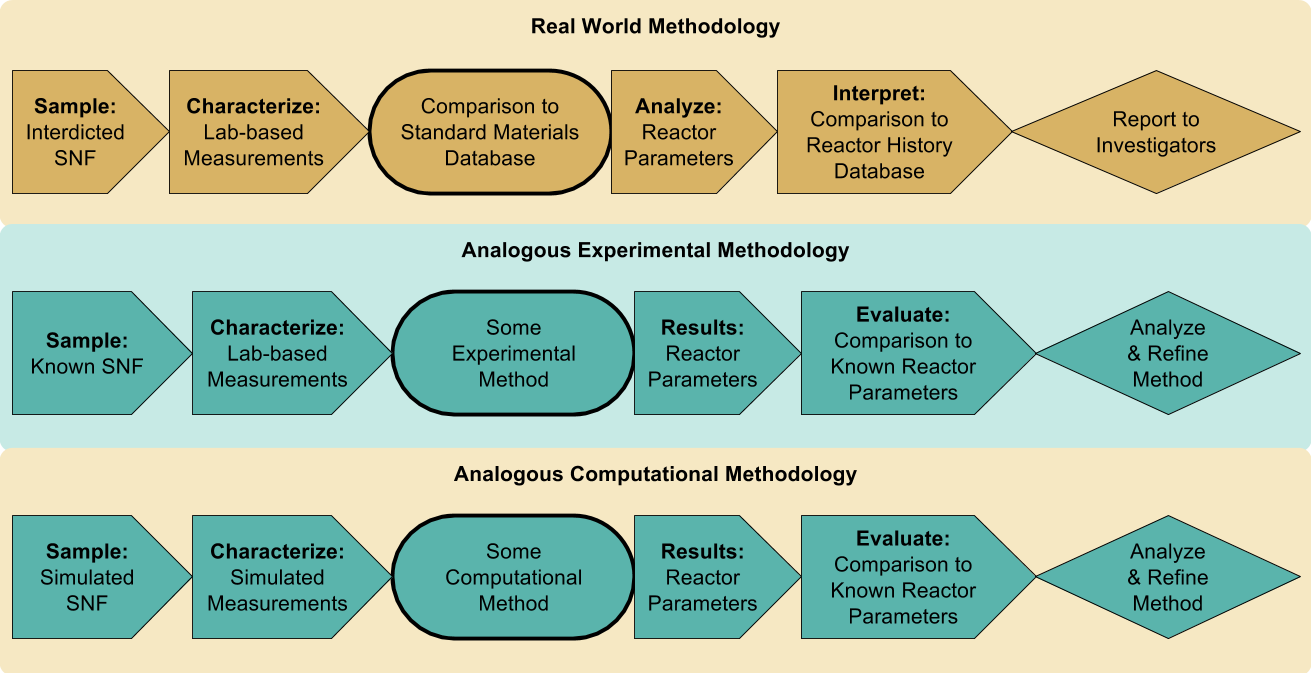
\includegraphics[width=0.9\textwidth]{./figures/ForensicsWorkflows.png}
    \caption{Nuclear forensics research: physical, experimental, and computational}
  \end{figure}
\end{frame}

\begin{frame}
  \frametitle{Computational Methods}
  \begin{figure}[h!]
    \centering
    \includegraphics[width=0.9\textwidth]{./figures/CompStatForensicsWorkflow.png}
    \caption{Comparison of two different computational approaches}
  \end{figure}
\end{frame}

\begin{frame}
  \frametitle{Statistical Methods}
  \begin{minipage}{0.5\textwidth}
    \begin{figure}
      \centering
      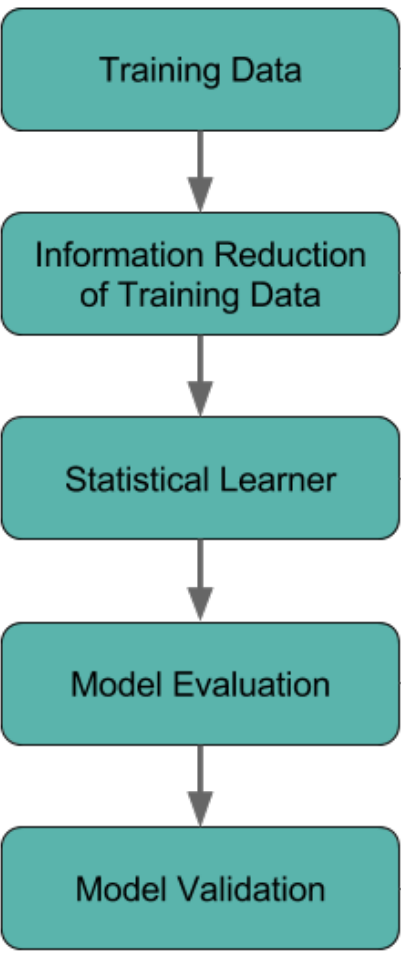
\includegraphics[height=0.6\textheight]{./figures/statmethodology.png}
      \caption{Workflow of a  methodology using statistical models}
    \end{figure}
  \end{minipage}%
  \begin{minipage}{0.5\textwidth}
    \begin{itemize}
      \item Training data: large set of SNF measurements
      \begin{itemize}
        \item Labels (e.g., burnup)
        \item Features (e.g., nuclide concs)
        \item Instances (individual SNF recipe)
      \end{itemize}
      \item Statistical learner
      \begin{itemize}
        \item Machine learning algorithms
        \item Algorithm parameters
        \item Predict label of new instance
      \end{itemize}
      \item Model evaluation
      \begin{itemize}
        \item Diagnostic curves
        \begin{itemize}
          \item Learning curves
          \item Validation curves
        \end{itemize}
        \item Prediction error
        \begin{itemize}
          \item Bias versus variance
          \item Generalizability
        \end{itemize}
      \end{itemize}
    \end{itemize}
  \end{minipage}
\end{frame}

\begin{frame}
  \frametitle{Statistical Methods}
  \begin{figure}[h!]
    \centering
    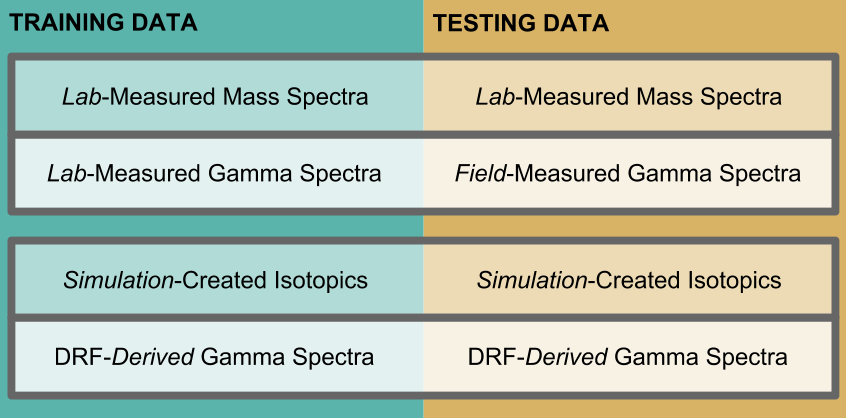
\includegraphics[width=0.75\textwidth]{./figures/proposal.png}
    \caption{Illustration of data set modularity}
  \end{figure}
\end{frame}



%% Do you have appendices?  If so, add them here, just like chapters.
% \begin{appendices}
% \include{backmatter/appendix1}
% \end{appendices}

%% McBride is a very nice style (some version is included in this distribution)
\bibliographystyle{mcbride}
\bibliography{dissertation}

\end{document}
